\documentclass{standalone}
\usepackage{tikz}
\begin{document}

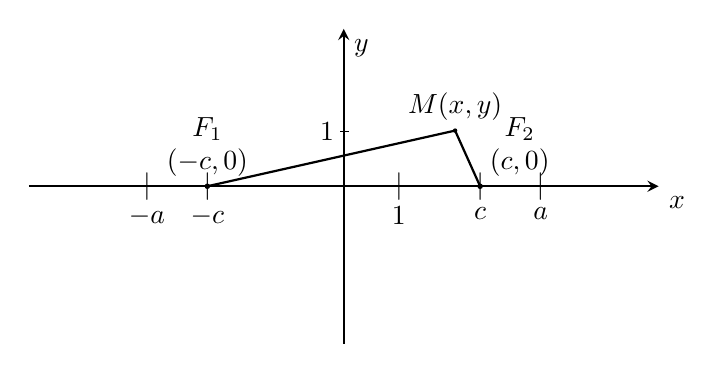
\begin{tikzpicture}[scale=1]

% Axes
\draw [thick, >=stealth, ->] (-4, 0) - -(4, 0)node[below right]{$x$};
\draw [thick, >=stealth, ->] (0, -2) - -(0, 2)node[below right]{$y$};

% Ellipe
\coordinate (F1) at (1.732,0);
\coordinate (F2) at (-1.732,0);
\coordinate (M) at ({2*cos(45)},{sin(45)});

\draw[thick] (M) node[above]{$M(x,y)$} -- (F2);
\draw[thick] (M) -- (F1);
\fill (M)circle (0.8pt);
\fill (F2) circle (1pt) 
      node[above, align=center] {$F_1$\\$(-c,0)$};
\fill (F1) circle (1pt) 
      node[above right, align=center] {$F_2$\\$(c,0)$};
\draw (F1)node{$|$};
\draw (F1)node[below, yshift=-4pt]{$c$};
\draw (F2)node{$|$};
\draw (F2)node[below, yshift=-4pt]{$-c$};
\draw (0,0.7)node{\_};
\draw (0,0.7)node[left]{1};
\draw (0.7,0)node{$|$};
\draw (0.7,0)node[below, yshift=-4pt]{1};
\draw (2.5,0)node{$|$};
\draw (2.5,0)node[below, yshift=-4pt]{$a$};
\draw (-2.5,0)node{$|$};
\draw (-2.5,0)node[below, yshift=-4pt]{$-a$};

\end{tikzpicture}


\end{document}